% Options for packages loaded elsewhere
\PassOptionsToPackage{unicode}{hyperref}
\PassOptionsToPackage{hyphens}{url}
\PassOptionsToPackage{dvipsnames,svgnames,x11names}{xcolor}
%
\documentclass[
  12pt,
]{interact}

\usepackage{amsmath,amssymb}
\usepackage{setspace}
\usepackage{iftex}
\ifPDFTeX
  \usepackage[T1]{fontenc}
  \usepackage[utf8]{inputenc}
  \usepackage{textcomp} % provide euro and other symbols
\else % if luatex or xetex
  \usepackage{unicode-math}
  \defaultfontfeatures{Scale=MatchLowercase}
  \defaultfontfeatures[\rmfamily]{Ligatures=TeX,Scale=1}
\fi
\usepackage{lmodern}
\ifPDFTeX\else  
    % xetex/luatex font selection
\fi
% Use upquote if available, for straight quotes in verbatim environments
\IfFileExists{upquote.sty}{\usepackage{upquote}}{}
\IfFileExists{microtype.sty}{% use microtype if available
  \usepackage[]{microtype}
  \UseMicrotypeSet[protrusion]{basicmath} % disable protrusion for tt fonts
}{}
\makeatletter
\@ifundefined{KOMAClassName}{% if non-KOMA class
  \IfFileExists{parskip.sty}{%
    \usepackage{parskip}
  }{% else
    \setlength{\parindent}{0pt}
    \setlength{\parskip}{6pt plus 2pt minus 1pt}}
}{% if KOMA class
  \KOMAoptions{parskip=half}}
\makeatother
\usepackage{xcolor}
\setlength{\emergencystretch}{3em} % prevent overfull lines
\setcounter{secnumdepth}{5}
% Make \paragraph and \subparagraph free-standing
\makeatletter
\ifx\paragraph\undefined\else
  \let\oldparagraph\paragraph
  \renewcommand{\paragraph}{
    \@ifstar
      \xxxParagraphStar
      \xxxParagraphNoStar
  }
  \newcommand{\xxxParagraphStar}[1]{\oldparagraph*{#1}\mbox{}}
  \newcommand{\xxxParagraphNoStar}[1]{\oldparagraph{#1}\mbox{}}
\fi
\ifx\subparagraph\undefined\else
  \let\oldsubparagraph\subparagraph
  \renewcommand{\subparagraph}{
    \@ifstar
      \xxxSubParagraphStar
      \xxxSubParagraphNoStar
  }
  \newcommand{\xxxSubParagraphStar}[1]{\oldsubparagraph*{#1}\mbox{}}
  \newcommand{\xxxSubParagraphNoStar}[1]{\oldsubparagraph{#1}\mbox{}}
\fi
\makeatother


\providecommand{\tightlist}{%
  \setlength{\itemsep}{0pt}\setlength{\parskip}{0pt}}\usepackage{longtable,booktabs,array}
\usepackage{calc} % for calculating minipage widths
% Correct order of tables after \paragraph or \subparagraph
\usepackage{etoolbox}
\makeatletter
\patchcmd\longtable{\par}{\if@noskipsec\mbox{}\fi\par}{}{}
\makeatother
% Allow footnotes in longtable head/foot
\IfFileExists{footnotehyper.sty}{\usepackage{footnotehyper}}{\usepackage{footnote}}
\makesavenoteenv{longtable}
\usepackage{graphicx}
\makeatletter
\def\maxwidth{\ifdim\Gin@nat@width>\linewidth\linewidth\else\Gin@nat@width\fi}
\def\maxheight{\ifdim\Gin@nat@height>\textheight\textheight\else\Gin@nat@height\fi}
\makeatother
% Scale images if necessary, so that they will not overflow the page
% margins by default, and it is still possible to overwrite the defaults
% using explicit options in \includegraphics[width, height, ...]{}
\setkeys{Gin}{width=\maxwidth,height=\maxheight,keepaspectratio}
% Set default figure placement to htbp
\makeatletter
\def\fps@figure{htbp}
\makeatother

\usepackage{booktabs}
\usepackage{longtable}
\usepackage{array}
\usepackage{multirow}
\usepackage{wrapfig}
\usepackage{float}
\usepackage{colortbl}
\usepackage{pdflscape}
\usepackage{tabu}
\usepackage{threeparttable}
\usepackage{threeparttablex}
\usepackage[normalem]{ulem}
\usepackage{makecell}
\usepackage{xcolor}
\usepackage{orcidlink}
\makeatletter
\@ifpackageloaded{caption}{}{\usepackage{caption}}
\AtBeginDocument{%
\ifdefined\contentsname
  \renewcommand*\contentsname{Table of contents}
\else
  \newcommand\contentsname{Table of contents}
\fi
\ifdefined\listfigurename
  \renewcommand*\listfigurename{List of Figures}
\else
  \newcommand\listfigurename{List of Figures}
\fi
\ifdefined\listtablename
  \renewcommand*\listtablename{List of Tables}
\else
  \newcommand\listtablename{List of Tables}
\fi
\ifdefined\figurename
  \renewcommand*\figurename{Figure}
\else
  \newcommand\figurename{Figure}
\fi
\ifdefined\tablename
  \renewcommand*\tablename{Table}
\else
  \newcommand\tablename{Table}
\fi
}
\@ifpackageloaded{float}{}{\usepackage{float}}
\floatstyle{ruled}
\@ifundefined{c@chapter}{\newfloat{codelisting}{h}{lop}}{\newfloat{codelisting}{h}{lop}[chapter]}
\floatname{codelisting}{Listing}
\newcommand*\listoflistings{\listof{codelisting}{List of Listings}}
\makeatother
\makeatletter
\makeatother
\makeatletter
\@ifpackageloaded{caption}{}{\usepackage{caption}}
\@ifpackageloaded{subcaption}{}{\usepackage{subcaption}}
\makeatother

\ifLuaTeX
  \usepackage{selnolig}  % disable illegal ligatures
\fi
\usepackage[]{natbib}
\bibliographystyle{plainnat}
\usepackage{bookmark}

\IfFileExists{xurl.sty}{\usepackage{xurl}}{} % add URL line breaks if available
\urlstyle{same} % disable monospaced font for URLs
\hypersetup{
  pdftitle={My wonderful paper},
  pdfauthor={H. Sherry Zhang; Roger D. Peng},
  colorlinks=true,
  linkcolor={blue},
  filecolor={Maroon},
  citecolor={Blue},
  urlcolor={Blue},
  pdfcreator={LaTeX via pandoc}}


\title{My wonderful paper}
\author{H. Sherry Zhang$\textsuperscript{1}$, Roger D.
Peng$\textsuperscript{1}$}

\thanks{CONTACT: H. Sherry
Zhang. Email: \href{mailto:huize.zhang@austin.utexas.edu}{\nolinkurl{huize.zhang@austin.utexas.edu}}. Roger
D.
Peng. Email: \href{mailto:roger.peng@austin.utexas.edu}{\nolinkurl{roger.peng@austin.utexas.edu}}. }
\begin{document}
\captionsetup{labelsep=space}
\maketitle
\textsuperscript{1} Department of Statistics and Data
Sciences, University of Texas at Austin, Texas, United States
\begin{abstract}
In data analysis, unexpected results often prompt researchers to revisit
their procedures to identify potential issues. While experienced
researchers can often quickly diagnose problems by checking a few key
assumptions, others may struggle to identify the root causes. These
checked assumptions, or expectations, are typically informal, difficult
to trace, and rarely discussed in publications. In this paper, we
formalize these informal assumptions by framing them as binary
\emph{analysis validation checks}. We then introduce a procedure to
quantify how violations of these checks may lead to unexpected results
in the analysis. The procedure relies on simulations of the original
data and evaluates both accuracy and redundancy. Accuracy is calculated
through a binary classification metric, while redundancy is measured
using mutual information. We demonstrate this approach with a toy
example based on fitness step count data and a generalized linear model
example examining the effect of particulate matter air pollution on
daily mortality.
\end{abstract}


\setstretch{2}
README:

\begin{itemize}
\tightlist
\item
  \emph{Check for TODOs}, things inside ``{[}\ldots{]}'', other than
  references, are my comments
\item
  Literature review: Section \emph{diagnosing unexpected outcomes in
  data analysis}
\item
  \emph{Discussion} and \emph{Conclusion}
\item
  In Section \emph{Application}: provide more context on the
  PM10-mortality study and add reference of the {[}0, 0.005{]} PM10
  coefficient
\end{itemize}

\newpage

\section{Introduction}\label{introduction}

In data analysis, experienced researchers often rely on their prior
knowledge or domain expertise to quickly assess whether results align
with their expectations. When a result falls outside of this interval,
it prompts the researchers to investigate backwards on the data quality,
the analysis steps, or the assumptions made during the analysis process.
This mental process of where to diagnose unexpected outcomes is often
difficult to trace and discuss in publications. As a result, readers are
typically presented with the final outcomes of the analysis cycle where
the results and expectations are aligned, achieved either by refining
the analysis or updating the expectations based on statistical evidence
\citep{grolemund_cognitive_2014}. These missing pieces of information
provides little guidance for diagnosing issues in the analysis when the
same methodology is applied to a new dataset that produces different
outcomes. Similarly, when researchers with different background
knowledge view results that they find to be unexpected, it becomes
unclear whether discrepancies arise from differing expectations or from
the use of statistical techniques.

One might gain insight into analysts' thought processes by speaking with
them directly or watching them work via screencast videos they produce,
such as, TidyTuesday screencast videos or think-aloud type studies
\citep[e.g.][]{gu2024data}. However, direct observation of analysis is
not scalable and may not always be feasible; creating educational
screencast videos requires significant effort from the researchers.
Ideally, there could be a way to make expectations about data analysis
explicit and accessible to others. Even better, if the encoding were
machine-readable, we could analyze these expectations and learn from the
analysis itself. For example, we could answer questions about whether
the checks also apply to other researchers analyzing new data in the
same context, whether they reflect common practices in the field, or
whether they are specific to the data or analysis at hand.

The externalization of the data analysis process is a practice that has
potential to improve the trustworthiness of analyses in general and the
trustworthiness of subsequent products, such as machine learning models,
that may be built on such analyses. While publication of analysis code
and data is now a common a requirement for the sake of reproducibility
\citep{peng2011reproducible}, the publication code alone is often
insufficient for understanding the thought process behind an analysis.
Code corresponding to published analyses often reflect the final
decisions made about analysis and do not reveal the decisions or
assumptions made about the data processing. Thus, a reader looking at
published code can often be left with many questions about why certain
choices were made. Developing an approach to reveal some of this process
without requiring a reader to essentially reconstruct the analysis
process from the raw data would provide an improved basis for trusting
an analysis result \citep{peng2021reproducible}.

In this paper, we conceptualize these internal expectations and
assumptions as \emph{analysis validation checks}, which allows us to
examine the assumptions made during an analysis and to diagnose
unexpected outcomes. We then introduce a procedure that provides a
quantitative measure of how violations in a tree of analysis checks,
derived from individual checks, will lead to an unexpected result. The
procedure, based on simulations of the original data, calculates the
accuracy and redundancy of the analysis checks. Accuracy is determined
using binary classification metrics, precision and recall, from a logic
regression fit \citep{ruczinski_logic_2003}, while redundancy is
measured using mutual information. The proposed workflow offers a
numerical guarantee that the analysis will produce the expected results,
assuming the assumptions about the data generating mechanism hold.

The rest of the paper is organized as follows:
Section~\ref{sec-lit-review} reviews the concepts of diagnosing
unexpected outcomes and general data quality checks.
Section~\ref{sec-plan} introduces the concept of analysis validation
checks, illustrated with a toy example based on fitness step count data.
Section~\ref{sec-method} describes the procedure that quantifies how
analysis validation checks combined using logical operators can predict
unexpected outcomes in an analysis. Section~\ref{sec-pm10-mortality}
applies this procedure to a larger example that estimates the effect of
particulate matter air pollution on daily mortality.
Section~\ref{sec-discussion} discusses a few key considerations and
Section~\ref{sec-conclusion} concludes the paper.

\section{Related Work}\label{sec-lit-review}

\subsection{Diagnosing unexpected outcomes in data
analysis}\label{diagnosing-unexpected-outcomes-in-data-analysis}

The concept of framing data analysis as a sense-making process was
originally presented by \citep{grolemund_cognitive_2014} based on
seminal work by \citep{wild1999statistical}. Key to any sense-making
process is a model for the world (i.e.~expectations for what we might
observe) and observed data with which we can compare our expectations.
If there is a significant deviation between what we observe and our
expectations, then a data analysis must determine what is causing that
deviation. A naive approach would be to update our model for the world
to match the data, under the assumption that the initial expectation was
incorrect. However, experienced analysts know that the reality can be
more nuanced than that, with errors occurring in data collection or data
processing that can have an impact on final results.

The skill of diagnosing unexpected data analysis results is not one that
has received significant attention in the statistics literature. While
the concept of diagnosis is often embedded in model checking or data
visualization techniques, systematic approaches to identifying the root
cause of an unexpected analysis result are typically not presented
\citep{peng2022perspective}. \citep{peng_diagnosing_2021} proposed a
series of exercises for training students in data analysis to diagnose
different kinds of analysis problems such as coding errors or outliers.
They provide a systematic approach involving working backwards from the
analysis result to identify potential causes. There are parallels here
to the concept of debugging and testing in software engineering
\citep{donoghue2021teaching}. For example, \citep{li2019towards} found
that experienced engineers were generally able to identify problems in
code faster than novices, and that the ability to debug code required
knowledge that cut across different domains.

If it is true that the speed with which data analysts can identify
problems with an analysis is related to their experience working with a
given type of data, then there is perhaps room to improve the analytic
process by externalizing the aspects that an analyst learns through
experience. That way, inexperienced analysts could examine the thought
process of an experienced analyst and learn to identify factors that can
cause unexpected results to occur.

\subsection{Data analysis checks}\label{data-analysis-checks}

A substantial body of literature has addressed the definition of data
quality \citep[more]{8642813} and has developed frameworks that include
dimensions, attributes, and measures to evaluate and improve data
quality
\citep{cai2015challenges, wang1996beyond, 6204995, woodall2014classification}.
These frameworks are often used in information systems and database
management and support business decision-making in various industries.
For research purposes, high-quality data ensures the credibility of
scientific findings and supports reproducibility and re-usability in
future studies {[}ref{]}. With the growing prevalence of open data in
scientific research, the consumers or users of the data typically are no
longer the producers or collectors of the data who would have the full
knowledge of data in hand, prompting more interest towards data quality
checks in the data analysis process. In R, there are some packages, like
\texttt{skimr} \citep{skimr} and \texttt{dataMaid} \citep{dataMaid},
that provide basic data screening and reporting tools, while another
class of packages, e.g.~\texttt{assertr} \citep{assertr},
\texttt{validate} \citep{validate}, and \texttt{pointblank}
\citep{pointblank} focuses on providing data validation tools, allowing
users to define customized data quality checks based on the
applications.

The literature on data quality typically focuses on the intrinsic or
inherent quality of the data themselves, rather than the data's
relationship to any specific data analysis. So for example, if a column
in a data table is expecting numerical data, but we observe a character
value in one of the entries, then that occurrence would trigger some
sort of data quality check. This type of quality check can be triggered
without any knowledge of what the data will ultimately be used for.
However, for a given analysis, we may require specific aspects of the
data to be true because they affect the result being computed.
Conversely, certain types of poor quality data may have little impact on
the ultimate result of an analysis (e.g.~data that are missing
completely at random). Defining data quality in terms of what may affect
a specific analysis outcome or result has the potential to open new
avenues for defining data checks and for building algorithms for
optimizing the collection of checks defined for a specific analysis.

\section{Analysis validation checks}\label{sec-plan}

Expectations represent our understanding of certain aspects of the
analysis and the data, independent of the results of the analysis
itself. When observed outcomes deviate from these expectations, analysts
often revisit the analysis process to identify potential issues, refine
methods, or revise assumptions. Experienced analysts can typically
identify issues quickly and correct them on the spot, but they often do
so without discussing the underlying reasoning, making it harder for
less experienced researchers to learn and master these skills.

Here, we introduce the concept of \textbf{analysis validation checks},
which frame these expectations or assumptions as explicit checks that
return a TRUE or FALSE result given the data analyzed at hand. Inspired
by the concept of data validation checks (\citet{validate}), which are
designed to ensure that datasets meet expected formats and quality,
analysis validation checks reverse the approach: they validate the
assumptions about the data necessary for the analysis to produce the
\emph{expected results}, as defined by the analyst. The focus on
expected results allows the concept of analysis validation checks to
encompass a broad range of checks, such as data quality (i.e.~missing
data, how the data are structured), data distribution and outliers,
bivariate and multivariate relationships between variables, and other
contextual information.

Our proposed analysis validation checks provide insights into an
analyst's thought process and offer the following benefits:

\begin{enumerate}
\def\labelenumi{\arabic{enumi}.}
\tightlist
\item
  Serve as clear checkpoints to support the replication or application
  of methods to (new) data by programmatically communicating the
  requirements or assumptions made of the data;
\item
  Align assumptions among researchers from different domain backgrounds
  who may have different expectations about the data;
\item
  Improve analysis transparency, reproducibility, and trustworthiness by
  externalizing a key part of the analysis process; and
\item
  Quantify the effectiveness of analysis checks for predicting the
  expected outcome (see Section~\ref{sec-method});
\end{enumerate}

In addition to the above benefits, the development and publication of
analysis checks has the potential to help students, inexperienced
analysts, and junior researchers develop the skills needed to diagnose
unexpected analysis results for a given type of data because the
assumptions made about the data are made transparent. The analysis
checks can serve as a basis for new analysts to have conversations about
the data they are analyzing and to develop a better understanding of the
potential data generation process.

\subsection{A Toy Example}\label{sec-toy}

Consider a 30-day step count experiment in public health. Subjects are
instructed to walk at least 8,000 steps each day, with an expected
average of 9,000 steps, tracked by a step counter app. After 30 days, we
review the data and examine the number of steps taken each day. With
data of this nature, we may expect there to be occasional ``low'' days
due to factors such as forgetting to wear their watch or unfavorable
weather conditions limiting outdoor activities. We may also expect
``high'' days recorded after an outdoor hike or intense workout. Given
the requirements of the study, we expect that for a given subject there
would be no more than five days with step counts falling below the
8,000-step threshold (``invalid days''). If there were more than five
invalid days, the data from that subject would not be usable for the
study.

In this scenario, the outcome is that the number of days with a step
count below 8,000 and the expectation is that this outcome would take a
value no more than 5. If the expectation is violated, we can consider
the potential configurations of the data that could lead to such an
anomaly. To diagnose potential reasons why this outcome expectation
might fail, we can establish a few analysis validation checks in
anticipation of seeing the data. For example, if the average step count
is too low, this may suggest that the subject is incapable of taking the
required number of steps, potentially leading to the unexpected outcome.
Similarly, we can also check the quantile of the step count, if more
than a third of the days fall below 8,000, this could indicate an excess
of low-count days. Additionally, we may may expect the standard
deviation of the step count not to be overly large. These considerations
yield the following three analysis validation checks:

\begin{itemize}
\tightlist
\item
  test1: the test fails if the mean step count is below 8,200
\item
  test2: the test fails if the 30th percentile of the observed step
  counts is below 8,200
\item
  test3: the test fails if the standard deviation of the observed step
  counts exceeds 2,500.
\end{itemize}

The cutoff values chosen for these tests would presumably be chosen
based on prior experience with these kinds of data, but could also be
optimized using the method presented in the next section.

\phantomsection\label{cell-fig-step-count}
\begin{figure}[H]

\centering{

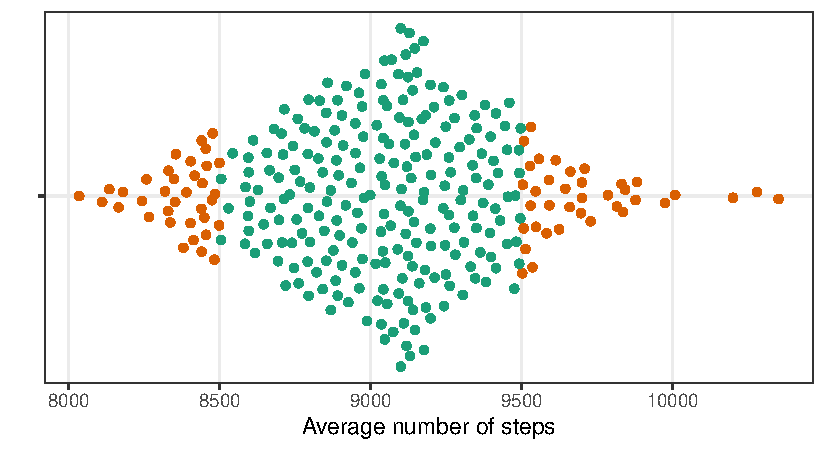
\includegraphics{index_files/figure-pdf/fig-step-count-1.pdf}

}

\caption{\label{fig-step-count}Number of days with fewer than 8,000
steps across 300 simulated 30-day periods. The orange bars indicate
instances where the count exceeds five days, representing an unexpected
outcome in this scenario.}

\end{figure}%

To simulate this data, three normal distributions are used for the daily
step counts: \(\mathcal{N}(4000, 200)\) for low days,
\(\mathcal{N}(12000, 200)\) for high days, and
\(\mathcal{N}(9000, 300)\) for typical days. The number of low and high
days can be simulated from a Poisson distribution with \(\lambda = 4\).
Figure~\ref{fig-step-count} displays the number of days with fewer than
8,000 steps across 300 simulated 30-day periods.

\section{Method}\label{sec-method}

While some checks may be crucial and directly indicate an unexpected
outcome, others may be tangential to the problem at hand and not
indicate a root cause of an unexpected outcome. In this section, we
propose a procedure to measure the effectiveness of checks that, when
combined using logical operators, contribute to an unexpected outcome. A
small set of independent checks is considered effective if it translates
to unexpected outcomes.

The approach relies on the use of simulated datasets that are generated
based on the analyst's knowledge and assumptions about the data
generation mechanism. Datasets are simulated to have the same structure
and characteristics of the observed data that will be analyzed at some
point in the future. For each simulated dataset, we can apply a
collection of analysis validation checks to the dataset and record which
ones were TRUE and which were FALSE. We can also compute the outcome of
the analysis to see whether the outcome is unexpected in a given
simulated datsets. We can then generate many datasets, each time
applying the analysis validation checks and computing the outcome. After
generating many datasets, we can relate the patterns in the analysis
validation checks to the likely that the outcome will be unexpected in a
given dataset. Figure~\ref{fig-metric-calc} provides an overview of the
process.

\phantomsection\label{cell-fig-metric-calc}
\begin{figure}[H]

\centering{

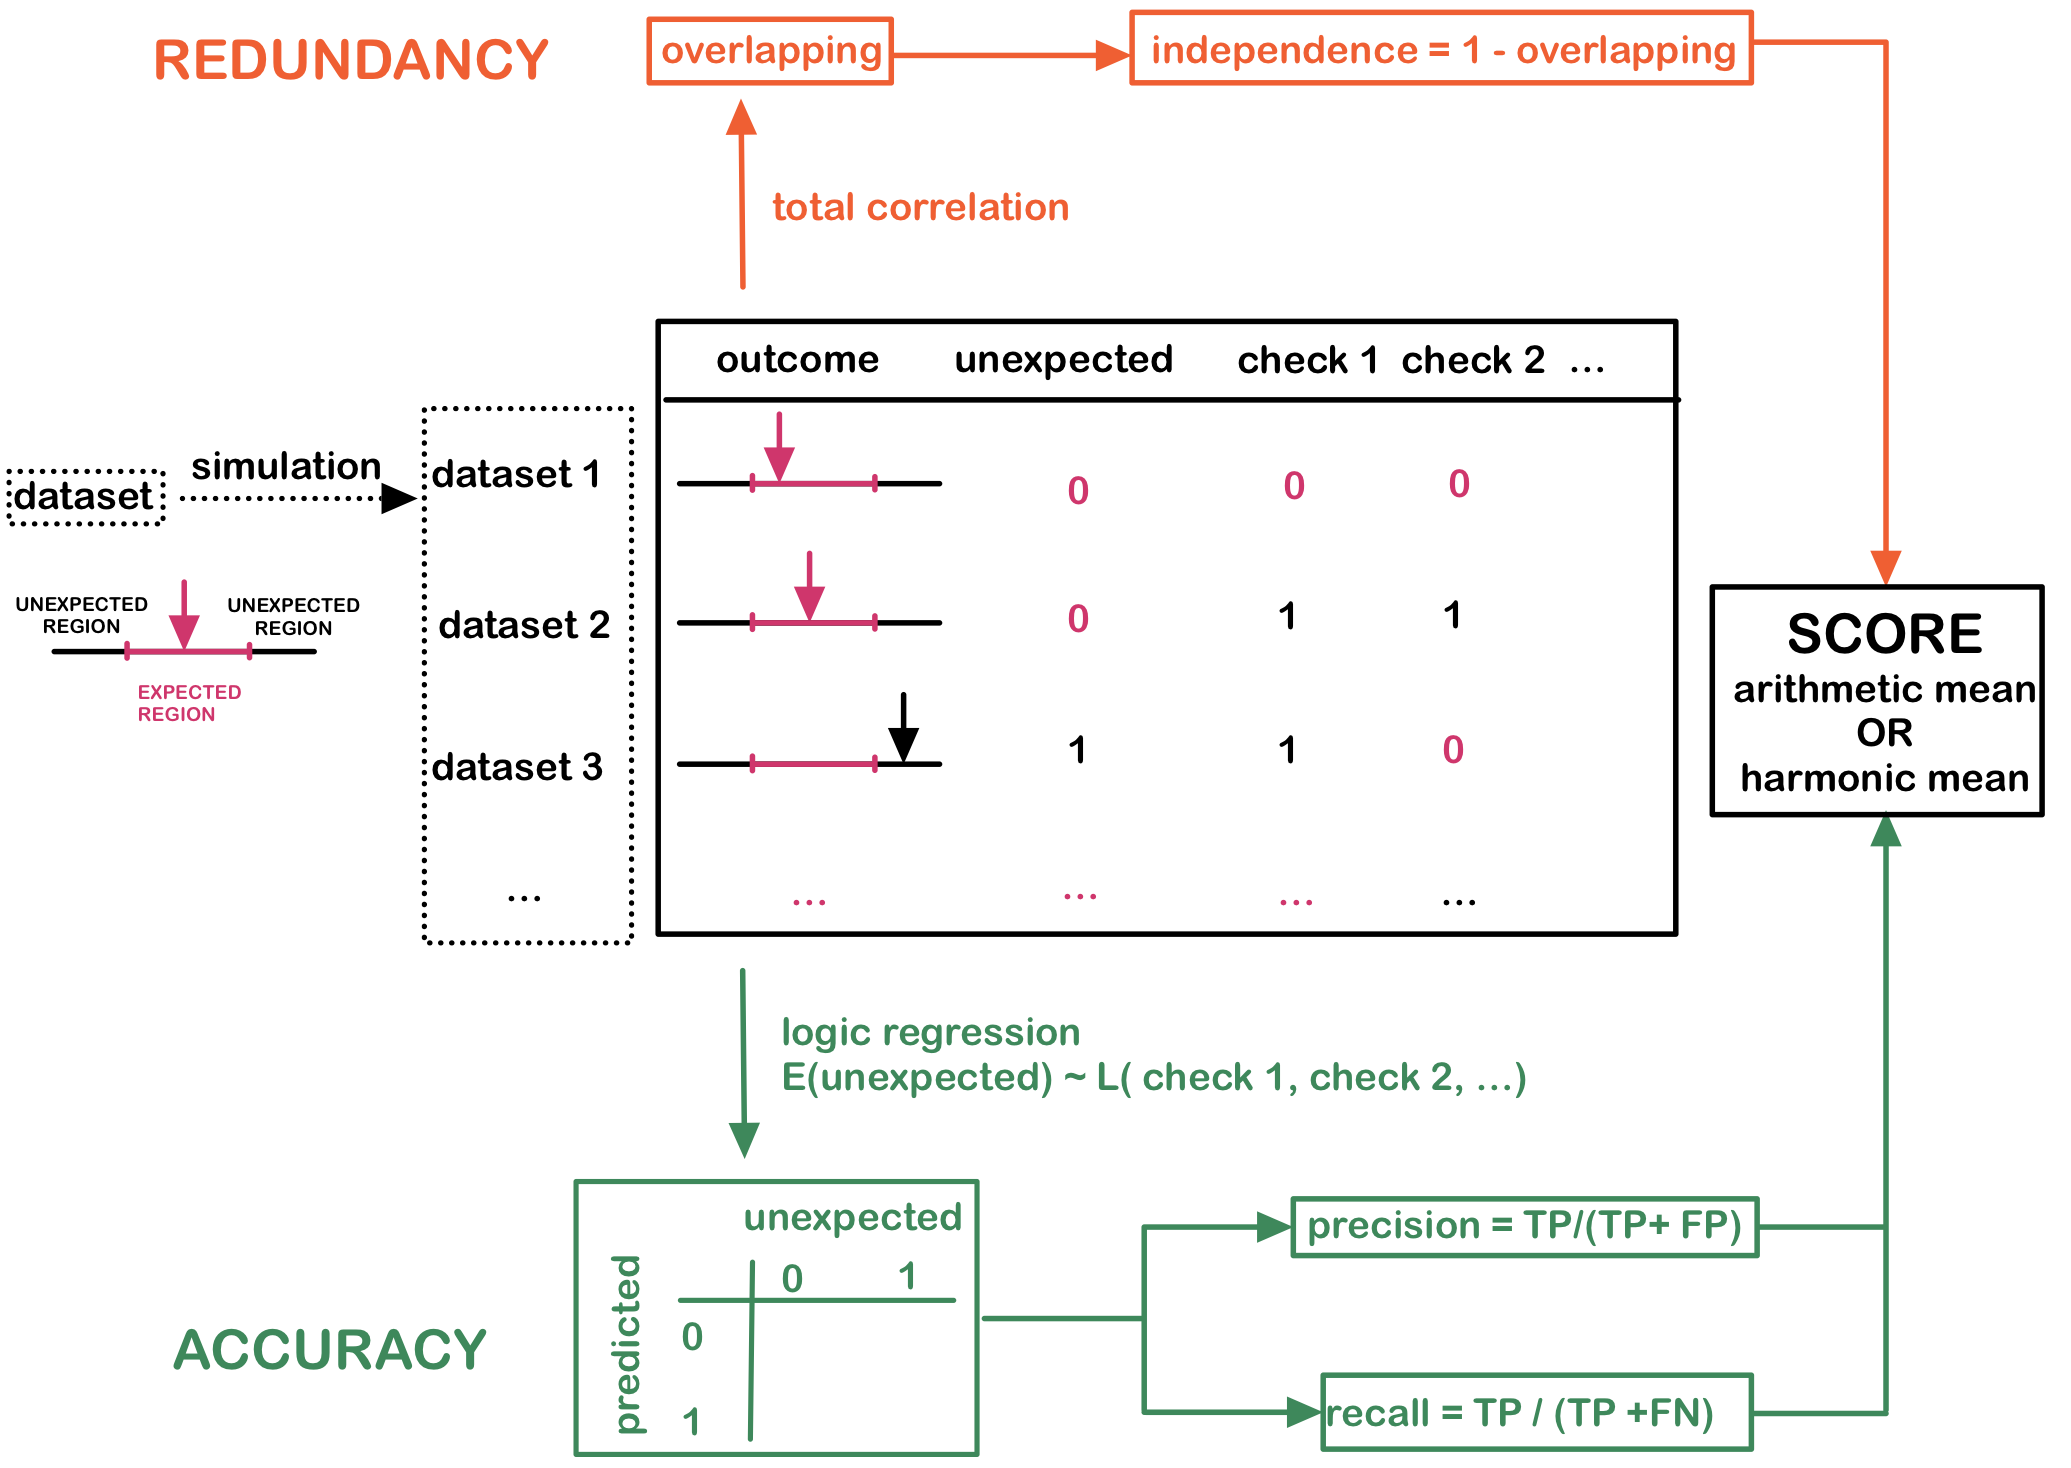
\includegraphics[width=6.73in,height=\textheight]{figures/metric-calc.png}

}

\caption{\label{fig-metric-calc}{[}this is the cap and the plot needs
polish{]}}

\end{figure}%

From the simulated data, the accuracy branch refers to a set of checks'
ability to accurately detect unexpected outcomes while minimizing false
positives and false negatives. While a false positive can raise caution
or skepticism on the data, the presence of both false positives and
false negatives suggest that the checks are overly sensitive or lack
sensitivity to unexpected outcomes.

To incorporate the effect of multiple checks on the outcome, a logic
regression model \citep{ruczinski_logic_2003} is fitted to the analysis
validation checks using the indicator of an unexpected result as the
outcome in the model. Originally developed for SNP microarray data,
logic regression constructs Boolean combinations of binary variables, in
a tree structure, to predict both binary and numerical outcomes.
Compared to other tree-based methods for binary-binary prediction, the
Boolean combinations from the logic regression model produce a tree
structure that can be directly interpreted as the possible combination
of checks leading to an unexpected outcome, without the need to invert
the tree as required in classic tree-based recursive partitioning
methods. The logic regression model is then used to predict the analysis
result based on the values of checks, and the prediction is compared to
the actual analysis result in order to calculate the precision and
recall of the checks.

While tests may score high on accuracy, they may be less effective at
explaining the various reasons behind unexpected results. This could
happen if, for example, a set of tests are all tangentially related to
the cause of the unexpected results, but none addresses the root cause.
It may also occur if the tests are highly correlated with one another,
leading to redundancy.

To quantify redundancy, the concept of mutual information is used.
Mutual information \(I(x, y)\) measures the amount of information shared
between two random variables and is defined as the KL-distance
\(D(p \parallel q)\) between the joint distribution of the two variables
and the product of the marginal distributions:

\[I(x,y) = D\big(p(x,y) \parallel p(x)p(y)\big) = \sum_x \sum_y p(x,y) \log \frac{p(x,y)}{p(x)p(y)}\]

This concept extends naturally to multiple variables through total
correlation, \(C(X_1, X_2, \cdots, X_n)\), which captures redundancy
across a set of \(n\) variables:

\[C(X_1, X_2, \cdots, X_n) = \sum_{x_1} \sum_{x_2} \cdots \sum_{x_n} p(x_1, x_2, \cdots, x_n) \log \frac{p(x_1, x_2, \cdots, x_n)}{p(x_1)p(x_2) \cdots p(x_n)}\]

A high mutual information value indicates redundancy among the tests,
while a low value suggests that the tests are independent and provides
unique information to diagnose the unexpected outcome. To standardize
this measure, the total correlation \emph{per observation} is
calculated, and an independence score, ranging between 0 and 1, is
defined as 1 - mutual information.

To combine precision, recall, and independence into a single metric, we
can combine the three scores using the arithmetic mean, harmonic mean,
or quadratic mean. The differences among these means are minimal when
the three metrics are similar. However, as the differences among the
metrics increases, the harmonic mean tends to produce the smallest
overall score, as it penalizes low values, while the quadratic mean
tends to produce the largest score by rewarding higher values more. For
simple interpretation of the score, the arithmetic mean is preferred,
while in applications where the difference between precision, recall,
and independence need to be penalized or rewarded more, the harmonic and
quadratic mean should be considered.

\subsection{Toy Example Revisited}\label{toy-example-revisited}

Returning to the step count example introduced in Section~\ref{sec-toy},
the logic regression model is fitted to the three analysis checks
described previously to generate the prediction of the unexpected
outcome, which is whether the number of days with fewer than 8,000 steps
is greater than 5. The predictions from the logic regression model can
be compared with the simulated true outcome for calculating the
precision and recall metrics. Figure~\ref{fig-logic-reg} shows the
best-fitting logic regression model, which is a combination of test1
(``mean step count is below 8,200'') and test3 (``standard deviation
exceeds 2,500'') with an OR operator. In other words, if either test1 or
test3 is true, then we would predict an unexpected outcome in the
analysis (i.e.~the number of days with fewer than 8,000 steps is greater
than 5).

\phantomsection\label{cell-fig-logic-reg}
\begin{figure}[H]

\centering{

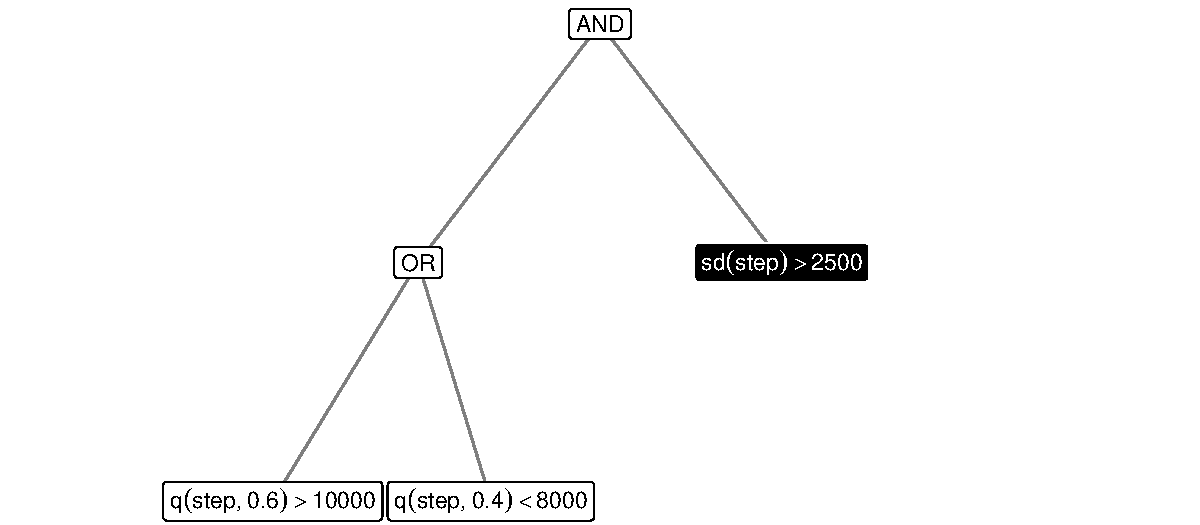
\includegraphics{index_files/figure-pdf/fig-logic-reg-1.pdf}

}

\caption{\label{fig-logic-reg}Logic regression model fitted to the three
unit tests (test1, test2, test3). The model suggests using an OR rule to
combine test1 and test3 to predict the outcome expectation.}

\end{figure}%

Table~\ref{tbl-logic-reg} presents the calculated precision, recall, and
independence for the three individual tests and the combined test rule
(test1 OR test3) from the logic regression. We also include the metric
calculated from fitting a regression tree model to the data to compare
the performance of the logic regression model. The harmonic and
arithmetic means are included to combine the three measures. The results
show that the two tests produced by the logic regression can accurately
predict 83.6\% cases of all \emph{actual unexpected results} in the
simulation data. Furthermore, 82.1\% of all \emph{predicted unexpected
results} were in fact observed to be unexpected.

\begin{longtable}[]{@{}
  >{\raggedright\arraybackslash}p{(\columnwidth - 10\tabcolsep) * \real{0.2424}}
  >{\raggedleft\arraybackslash}p{(\columnwidth - 10\tabcolsep) * \real{0.1515}}
  >{\raggedleft\arraybackslash}p{(\columnwidth - 10\tabcolsep) * \real{0.1061}}
  >{\raggedleft\arraybackslash}p{(\columnwidth - 10\tabcolsep) * \real{0.1970}}
  >{\raggedleft\arraybackslash}p{(\columnwidth - 10\tabcolsep) * \real{0.1364}}
  >{\raggedleft\arraybackslash}p{(\columnwidth - 10\tabcolsep) * \real{0.1667}}@{}}

\caption{\label{tbl-logic-reg}Accuracy (precision and recall) and
parsimony (independence) metrics for each individual unit test and for
the combined test rule (test1 OR test3) derived from the logic
regression model. The harmonic and arithmetic means of the three metrics
are included to evaluate the quality of the unit tests in diagnosing
unexpected step counts (more than five days with fewer than 8,000
steps).}

\tabularnewline

\toprule\noalign{}
\begin{minipage}[b]{\linewidth}\raggedright
tests
\end{minipage} & \begin{minipage}[b]{\linewidth}\raggedleft
precision
\end{minipage} & \begin{minipage}[b]{\linewidth}\raggedleft
recall
\end{minipage} & \begin{minipage}[b]{\linewidth}\raggedleft
independence
\end{minipage} & \begin{minipage}[b]{\linewidth}\raggedleft
harmonic
\end{minipage} & \begin{minipage}[b]{\linewidth}\raggedleft
arithmetic
\end{minipage} \\
\midrule\noalign{}
\endhead
\bottomrule\noalign{}
\endlastfoot
test1 & 0.482 & 0.964 & 1.000 & 0.730 & 0.815 \\
test2 & 0.214 & 1.000 & 1.000 & 0.450 & 0.738 \\
test3 & 0.589 & 0.805 & 1.000 & 0.762 & 0.798 \\
test1 OR test3 & 0.821 & 0.836 & 0.999 & 0.879 & 0.886 \\
regression tree & 0.821 & 0.836 & 1.000 & 0.879 & 0.886 \\

\end{longtable}

For comparison, the regression tree produces a similar prediction to the
logic regression, by first splitting on test1 and then splitting on
test3, and results in the same accuracy and overall score as the logic
regression model. However, we argue that the logic regression tree shown
in Figure~\ref{fig-logic-reg} is more interpretable for our purposes
because it provides a direct representation of which combinations of
analysis checks lead to unexpected outcomes. The logic regression tree
is also directly comparable to other diagnostic techniques, which we
discuss further in Section~\ref{sec-discussion}.

\section{Application}\label{sec-pm10-mortality}

In the study of the health effects of outdoor air pollution, one area of
interest is the association between short-term, day-to-day changes in
particulate matter air pollution and daily mortality counts. Substantial
work has been done to study this question and to date, there appears to
be strong evidence of an association between particulate matter less
than 10 \(\mu\)g/m\(^3\) in aerodynamic diameter (PM10) and daily
mortality from all non-accidental causes \citep{samet2000fine}. For our
second example, we use the problem of studying PM10 and mortality along
with data from the National Morbidity, Mortality, and Air Pollution
Study (NMMAPS) to demonstrate how our analysis validation checks
described in Section~\ref{sec-method} can be applied.

The typical approach to studying the association between PM10 and
mortality is to apply a generalized linear model with a Poisson link to
relate daily mortality counts to daily measures of PM10. Based on
previous work and the range of effect sizes published in the literature,
an analyst might expect the coefficient for PM10 in this GLM to lie
between {[}0, 0.005{]}, after adjusting for daily temperature
\citep{samet200fine, welty2005acute}. Observing an estimated coefficient
outside of this interval would be highly unusual and would warrant a
serious re-examination of the analysis process. Therefore, our
unexpected outcome in this analysis will be the binary indicator of
whether the estimated coefficient for PM10 in the GLM lies outside of
the interval {[}0, 0.005{]}. In addition to providing a more substantial
problem for our methods, this example also demonstrates how the
procedure presented in Section~\ref{sec-method} can be used to select
cutoff values in the analysis checks to diagnose an unexpected PM10
coefficient from the generalized linear model.

This PM10 coefficient expectation can be framed as an analysis check
that fails, labelled as 1, if the estimate of the PM10 coefficient
(adjusted for temperature) is outside the range {[}0, 0.005{]}, and 0 if
it is within. Multiple factors can affect the estimated PM10
coefficient, such as the sample size, the strength of the correlation
between mortality and PM10, and the strength of the correlation between
mortality and temperature. Analysts may expect a reasonable sample size
to ensure the reliability of the coefficient estimate. Outliers in the
three variables can also leverage the coefficient. While these are
possible factors that could affect the analysis result, it is not clear
what the cutoff values for these checks should be to determine a
failure. Here we consider a list of checks in Table~\ref{tbl-checks}
with varied cutoff values for each:

\begin{longtable}[]{@{}l@{}}
\caption{A list of checks considered for the generalized linear model of
mortality on PM10 and temperature. The checks are based on the sample
size, correlation between mortality and PM10, correlation between
mortality and temperature, and univariate outlier detection. Multiple
cutoff values are specified for each check to determine a
failure.}\label{tbl-checks}\tabularnewline
\toprule\noalign{}
the check fails if \ldots{} \\
\midrule\noalign{}
\endfirsthead
\toprule\noalign{}
the check fails if \ldots{} \\
\midrule\noalign{}
\endhead
\bottomrule\noalign{}
\endlastfoot
Sample size less than or equal to 200 \\
Sample size less than or equal to 400 \\
Sample size less than or equal to 600 \\
Sample size less than or equal to 800 \\
Mortality-PM10 correlation less than -0.03 \\
Mortality-PM10 correlation less than -0.04 \\
Mortality-PM10 correlation less than -0.05 \\
Mortality-PM10 correlation less than -0.06 \\
Mortality-temperature correlation greater than -0.3 \\
Mortality-temperature correlation greater than -0.35 \\
Mortality-temperature correlation greater than -0.4 \\
Mortality-temperature correlation greater than -0.45 \\
Outlier(s) are presented in the variable PM10 \\
Outlier(s) are presented in the variable mortality \\
\end{longtable}

\subsection{Data Simulation}\label{data-simulation}

To generate replicates of the dataset, we first generate the correlation
matrix of the three variables (PM10, mortality, and temperature) in a
grid and then use a Gaussian copula to generate a multivariate normal
distribution based on the specified correlation matrix and sample size.
The multivariate normal distribution is transformed using the normal CDF
before the inverse CDF of the assumed distributions of the three
variables is applied. To determine the appropriate distribution of each
variable, various distributions are fitted and compared. This includes
poisson and negative binomial for mortality; gamma, log-normal,
exponential, weibull, and normal for PM10 and temperature; and beta for
PM10 after rescaling the data to \([0,1]\).

To ensure a reasonable likeness to data that might be used in such an
analysis, we use characteristics of the observed dataset to refine our
simulations. AIC is used to determine the best distribution fit for each
variable with the QQ-plot presented in Figure~\ref{fig-dist-fit} to
evaluate the fit. AIC suggests a negative binomial distribution for
mortality, a beta distribution for PM10 (multiple by 100 to recover the
original scale), and a Weibull distribution for temperature. To include
the potential effect of outliers, we add a single outlier to the data
for both the mortality and PM10 variables.

\phantomsection\label{cell-fig-dist-fit}
\begin{figure}[H]

\centering{

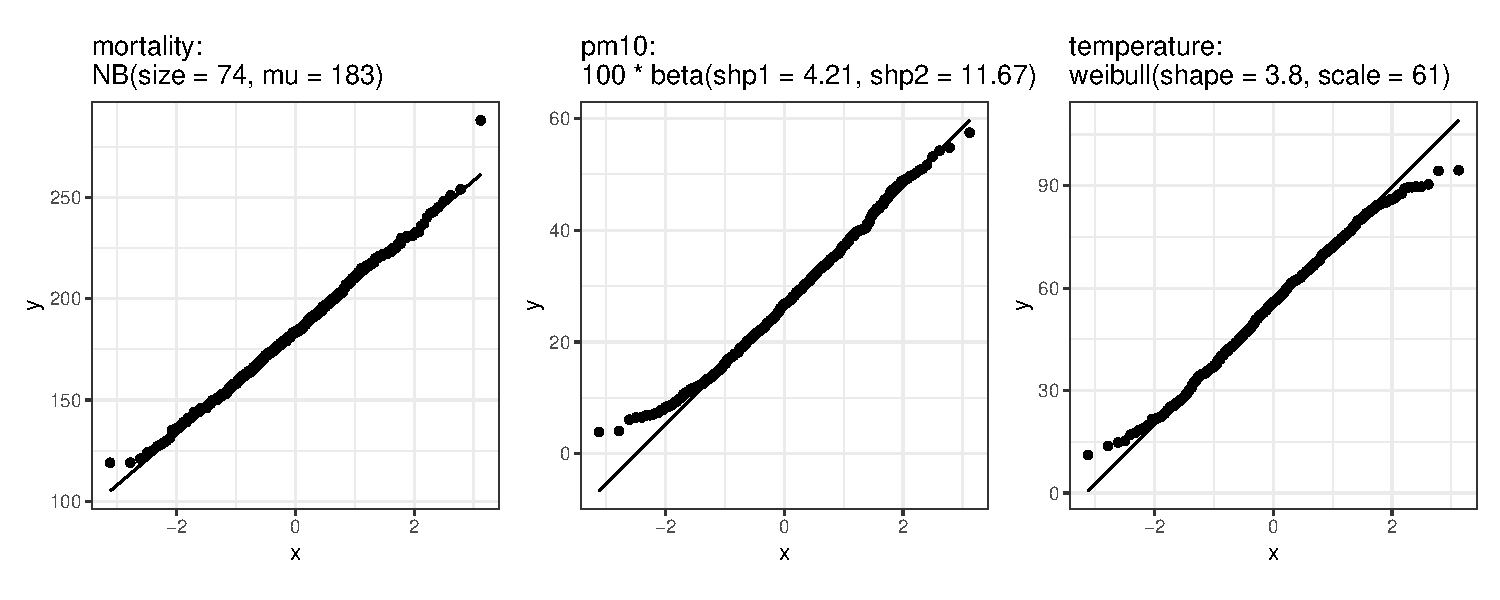
\includegraphics{index_files/figure-pdf/fig-dist-fit-1.pdf}

}

\caption{\label{fig-dist-fit}QQ-plot of the distribution fit for
mortality, PM10, and temperature based on the fitted distribution from
the original data. The fitted distribution is compared to the observed
data to assess the distribution fit.}

\end{figure}%

A logic regression is fitted using all variations of the tests in
Table~\ref{tbl-checks} to predict whether the PM10 coefficient is
unexpected. Figure~\ref{fig-linear-reg-tree} shows the optimal logic
regression tree from the fitted model. Precision, recall, and
independence score, along with their harmonic and arithmetic mean are
calculated in Table~\ref{tbl-linear-reg}.

\begin{figure}

\centering{

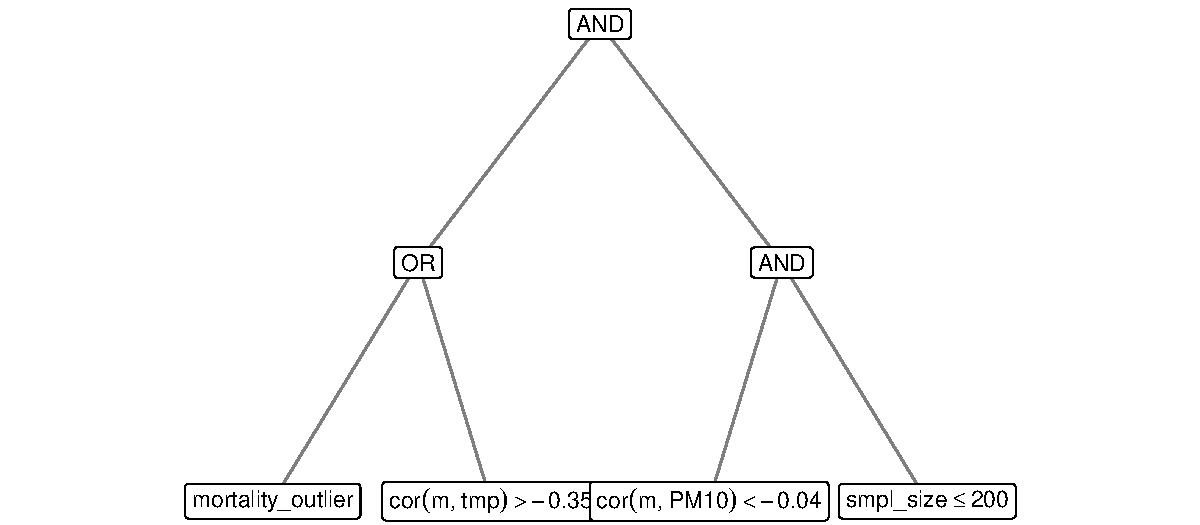
\includegraphics{index_files/figure-pdf/unnamed-chunk-8-1.pdf}

}

\caption{\label{fig-linear-reg-tree}Logic regression model fitted to the
fourteen unit tests and the outcome expectation (unexpected) as the
response variable. The model suggests the relationship: (sample size
\emph{greater than} 200 AND mortality-PM10 correlation \textless{}
-0.04) AND (mortality-temperature correlation \textgreater{} -0.35 OR
there exist mortality outlier) to predict the unexpected PM10
coefficient. {[}sorry the proper plot is not ready{]}.}

\end{figure}%

\begin{longtable}[]{@{}
  >{\raggedleft\arraybackslash}p{(\columnwidth - 12\tabcolsep) * \real{0.0882}}
  >{\raggedleft\arraybackslash}p{(\columnwidth - 12\tabcolsep) * \real{0.1471}}
  >{\raggedleft\arraybackslash}p{(\columnwidth - 12\tabcolsep) * \real{0.1029}}
  >{\raggedleft\arraybackslash}p{(\columnwidth - 12\tabcolsep) * \real{0.1765}}
  >{\raggedleft\arraybackslash}p{(\columnwidth - 12\tabcolsep) * \real{0.1912}}
  >{\raggedleft\arraybackslash}p{(\columnwidth - 12\tabcolsep) * \real{0.1324}}
  >{\raggedleft\arraybackslash}p{(\columnwidth - 12\tabcolsep) * \real{0.1618}}@{}}

\caption{\label{tbl-linear-reg}Accuracy (precision and recall) and
parsimony (independence) metrics derived from the logic regression
model, along with harmonic and arithmetic means, for individual unit
tests (1: sample size, 2: mortality-PM10 correlation, 3:
mortality-temperature correlation, 4: mortality outlier), and the
combined test rule 5: (sample size AND mortality-PM10 correlation) AND
(mortality-temperature correlation OR mortality outlier.}

\tabularnewline

\toprule\noalign{}
\begin{minipage}[b]{\linewidth}\raggedleft
tests
\end{minipage} & \begin{minipage}[b]{\linewidth}\raggedleft
precision
\end{minipage} & \begin{minipage}[b]{\linewidth}\raggedleft
recall
\end{minipage} & \begin{minipage}[b]{\linewidth}\raggedleft
overlapping
\end{minipage} & \begin{minipage}[b]{\linewidth}\raggedleft
independence
\end{minipage} & \begin{minipage}[b]{\linewidth}\raggedleft
harmonic
\end{minipage} & \begin{minipage}[b]{\linewidth}\raggedleft
arithmetic
\end{minipage} \\
\midrule\noalign{}
\endhead
\bottomrule\noalign{}
\endlastfoot
1 & 0.087 & 0.215 & 0 & 1 & 0.175 & 0.434 \\
2 & 0.988 & 0.610 & 0 & 1 & 0.822 & 0.866 \\
3 & 0.392 & 0.581 & 0 & 1 & 0.569 & 0.658 \\
4 & 0.649 & 0.641 & 0 & 1 & 0.732 & 0.763 \\
5 & 0.760 & 0.880 & 0 & 1 & 0.869 & 0.880 \\

\end{longtable}

As indicated in Figure~\ref{fig-linear-reg-tree}, the logic regression
model picks up the following cutoff values for each type of check:

\begin{itemize}
\tightlist
\item
  sample size \emph{larger than} 200
\item
  mortality-temperature correlation greater than \(-0.35\)
\item
  mortality-PM10 correlation less than \(-0.04\)
\item
  mortality data contains outliers that are detected by the univariate
  outlier detection
\end{itemize}

The tree structure suggests checking mortality-PM10 correlation and a
sample size larger than 200 with an additional check of either outlier
on mortality or correlation between mortality and temperature. This
combined check rule generates a precision of 0.76 and a recall of 0.88
for predicting the unexpected PM10 coefficient. The single check,
\texttt{cor(m,\ PM10)\ \textless{}\ -0.03}, is also powerful with a high
precision of 0.988, but the low recall value of 0.61 suggests its high
false positive rate, as compared to the combined rule suggested by the
logic regression.

As shown in Figure~\ref{fig-linear-reg-tree}, there is no single
analysis check in the tree that predicts an unexpected outcome. rather
at least three checks in the tree must be TRUE in order for the model to
predict an unexpected outcome. Given the high independence of the tests
(Table~\ref{tbl-linear-reg}), this suggests that unexpected results are
only likely after multiple anomalies are observed in the data.

\section{Discussion}\label{sec-discussion}

In this paper we have developed an approach to using analysis validation
checks to externalize the assumptions about the data and analysis tools
made during the data analysis process. These checks can serve as a
useful summary of the analyst's thought process and can desscribe how
characterstics of the data may lead to unexpected outcomes. Using logic
regression, we can develop a graphical summary of the analysis
validation checks as well as use the logic regression fitting process to
choose the optimal set of checks. The logic regression model can also be
used to develop summaries of the precision and recall of the collection
of analysis validation checks in predicting the likelihood of an
unexpected outcome. We demonstrated our method on an example relating
daily mortality to outdoor air pollution data.

An interesting connection can be drawn between our logic regression
trees and a tool used in systems engineering known as a fault tree. A
fault tree is used for conducting a structured risk assessment and has a
long history in aviation, aerospace, and nuclear power applications
\citep{vesely1981fault}. A fault tree is a graphical tool that describes
the possible combinations of causes and effects that lead to an anomaly.
At the top of the tree is a description of an anomaly. The subsequent
branches of the tree below the top event indicate possible causes of the
event immediately above it in the tree. The tree can then be built
recursively until we reach a root cause that cannot be further
investigated. Each level of the tree is connected together using logic
gates such as AND and OR gates. The leaf nodes of the tree indicate the
root causes that may lead to an anomaly. While the logic regression
tress are not identical to fault trees, they share many properties, such
as the tree-based structure and the indicator of root causes at the leaf
nodes. Perhaps more critically, both serve as graphical summaries of the
assumptions made in a problem and the specific violations of those
assumptions that could lead to an unexpected result. While fault trees
are often used to discover the root cause of an anomaly after it occurs,
an important use case for fault trees is to develop a comprehensive
understanding of a system \emph{before} an anomaly occurs
\citep{michael2002fault}.

TODO

\begin{itemize}
\item
  how to systematically simulate data is still unknown
\item
  plotting is a critical way to check data and they can still be frame
  into checks. i.e.~the density/ histogram suggests there are outliers.
  It is a open problem to how to encode the visualization into checks.
\item
  currently no automated way to generate checks. It is interesting to
  see how check generation can be automated, although it requires the
  inputs from experts across a wide array of common scenarios.
\item
  checks are also closely related to the concept of unit tests in
  software engineering. While unit tests are designed to isolate and
  test specific aspects of the code, it is difficult for analysis
  validation check to do so.
\item
  There are cost and benefit on setting expectation on different
  granularity. At the lowest level, one may have a plan for each data
  entry and every data handling steps. This requires more work from the
  analysts and may not be practical in practice. For more complex
  analyses, analysts may divide the analysis into sections and set
  expectations for each. They can then focus on the specific sections
  flagged by the tests and sub-divide the sections to set expectation
  and diagnose the analysis in a hierarchical manner.
\end{itemize}

\section{Conclusion}\label{sec-conclusion}

TODO

\section{Acknowledgement}\label{acknowledgement}

The article is created using Quarto \citep{Allaire_Quarto_2022} in R
\citep{R}. The source code for reproducing the work reported in this
paper can be found at:
\url{https://github.com/huizezhang-sherry/paper-avc}.


\renewcommand\refname{References}
  \bibliography{references.bib}



\end{document}
